%! Author = joaos
%! Date = 02/11/2024

\section*{Preparação e Caracterização de Amostras}

\newday{21 Outubro 2024}

Foi feito um trabalho de desagregação da amostra inicial, proveniente da mina do Numão.
Uma amostra de um pré-concentrado que tinha sido anteriormente submetida a processos de flutuação.
A amostra tinha cerca de 15~kg.

\begin{marginfigure}
    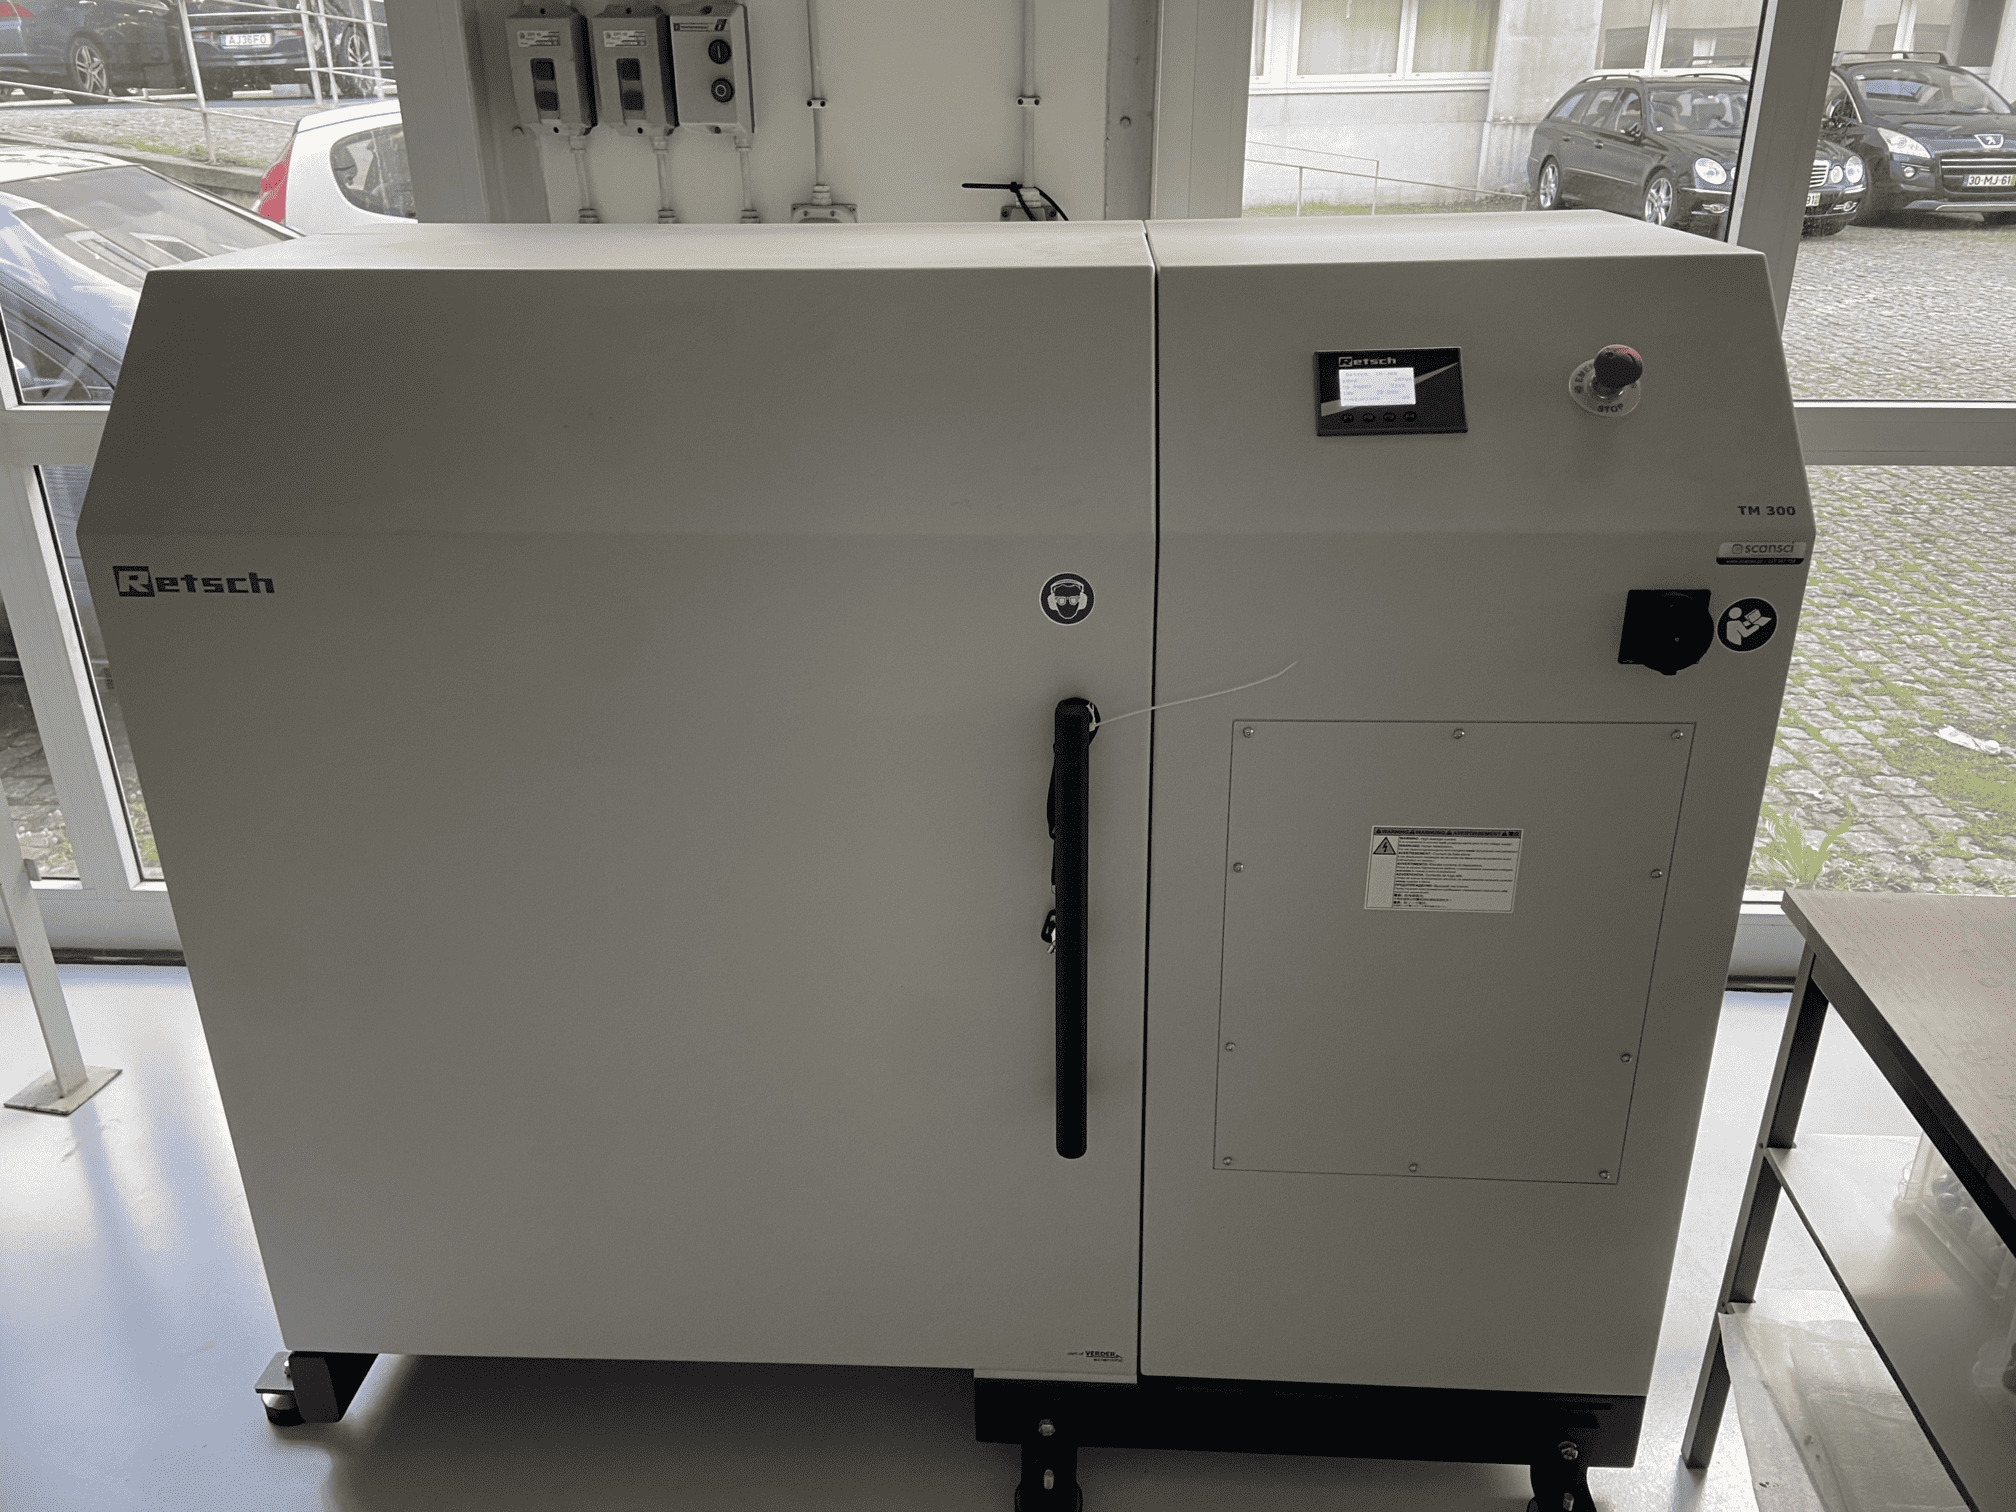
\includegraphics[width=\linewidth]{figures/moinho_tm300}
    \caption{Moinho de tambor \href{https://www.retsch.pt/pt/produtos/trituracao/moinhos-planetarios-e-de-bolas/tm-300/}{TM 300 Retsch}.}
    \label{fig:moinho_tm300}
\end{marginfigure}

Foi utilizado um moinho de bolas - apresentado na Figura~\ref{fig:moinho_tm300} - com a seguinte configuração de trabalho:
\begin{itemize}
    \item[-] 60 rpm;
    \item[-] Duração de trabalho 30~minutos;
\marginnote{Como o moinho nunca tinha sido utilizado para desagregar amostras, fez-se testes para determinar o tempo necessário de funcionamento e para determinar também a necessidade ou não de bolas.}
    \item[-] Sentido de rotação inverte de 5 em 5~minutos;
    \item[-] Pausa de 1~minuto entre cada inversão de sentido;
    \item[-] 3,41~kg de bolas.
\end{itemize}

Foi-se colocando partes da amostra dentro do tambor do moinho e deixou-se a desagregar durante o tempo estipulado.
\marginnote{O peneiro de \#1.18~mm foi utilizado como redundância, apenas para ter a certeza que toda a amostra estava desagregada.}
Uma vez terminado o tempo de funcionamento do moinho, peneirou-se o material desagregado com um peneiro de malha \#1.18~mm.
Foi-se fazendo este procedimento sucessivamente.
Deixou-se material para o dia seguinte.

\hrulefill

%%%%%%%%%%%%%%%%%%%%%%%%%%%%%%%%%%%%%%%%%%%%%%%%%%%%%%%%

\newday{22 Outubro 2024}

\textit{Na Figura~\ref{fig:amostra_no_moinho} temos a amostra de material dentro do tambor do moinho.}

\begin{marginfigure}
    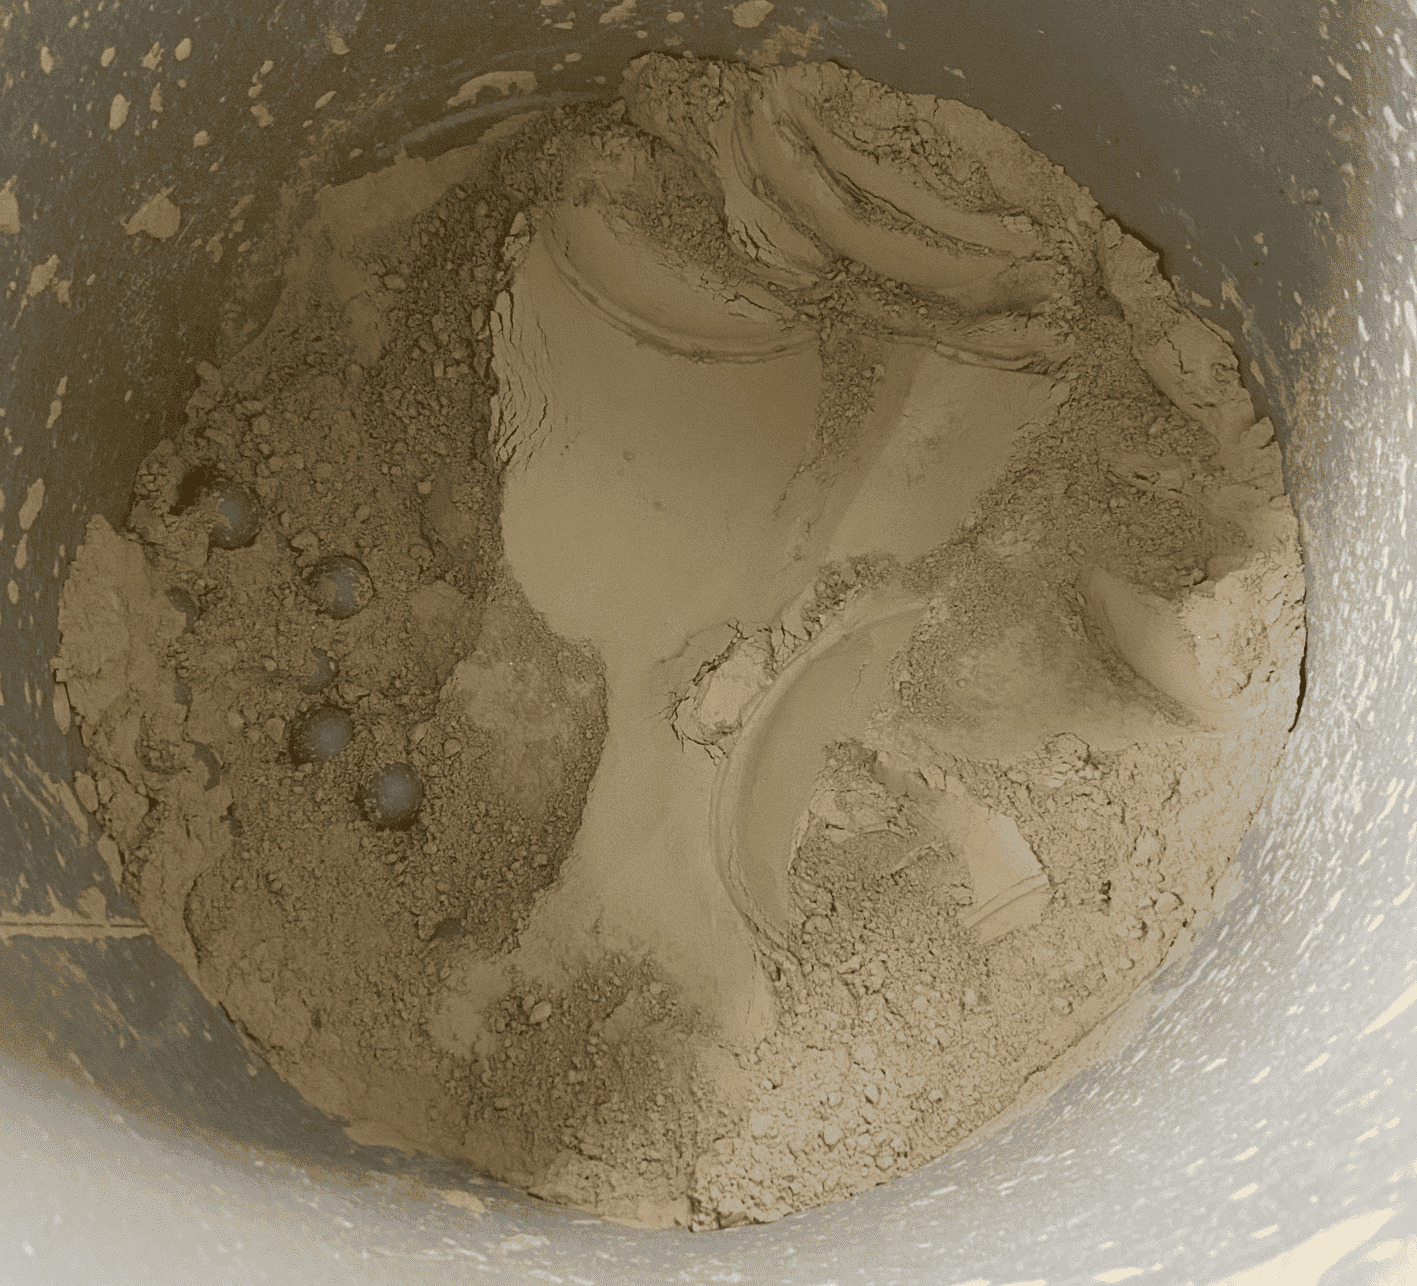
\includegraphics[width=\linewidth]{figures/amostra_no_moinho}
    \caption{Amostra de material no tambor do moinho.}
    \label{fig:amostra_no_moinho}
\end{marginfigure}

Do dia anterior verificou-se que ainda havia alguns ``blocos'', portanto meteu-se o moinho a trabalhar durante cerca de 15~minutos para desagregar o resto do material.
Quando este terminou, a totalidade da amostra foi desagregada e peneirada com o peneiro \#1.18~mm.

Com o material já desagregado, era necessário agora homogeneizar a amostra.
Para isso, foi utilizado o separador \emph{Jones}\sidenote{O separador \emph{Jones}, ou em inglês \emph{riffle splitter}, é utilizado para separar amostras em duas partes quase idênticas.} (esquartelador).
Separou-se a amostra de $\approx$~15~kg em duas amostras de $\approx$~7,5~kg cada - amostra A e amostra B\@.

A amostra B vai ser guardada.
Foi armazenada em dois sacos de plástico - B$_1$ = 3,36~kg e B$_2$ = 4,28~kg.
A amostra A será posteriormente separada em sacos de $\approx$~1~kg.

\hrulefill
\pagebreak
%%%%%%%%%%%%%%%%%%%%%%%%%%%%%%%%%%%%%%%%%%%%%%%%%%%%%%%%

\newday{24 Outubro 2024}

\textit{N.B.: Antes de se utilizar o separador \emph{Jones}, tinha sido feita uma separação manual. Esta abordagem não poderia estar mais errada, separar a amostra manualmente introduz erros significativos, especialmente em amostras com partículas de diferentes calibres. O Jones é uma das formas representativas e precisas de separação de amostras e é o que será utilizado neste trabalho.}

\marginnote{É importante ter em consideração que obtêm-se sempre duas amostras com o separador \textit{Jones}, mas que uma das metades obtidas é \textbf{sempre} descartada. Ou seja, na Figura~\ref{fig:diagrama_jones}, o ramo da direita de cada uma das ramificações foi descartado para ser separado posteriormente (a totalidade da amostra foi separada em sacos de $\approx$~1~kg).}

\subsection{Funcionamento do separador Jones}\label{subsec:funcionamento-do-separador-jones}

O \emph{Jones} separa uma amostra em duas metades, sendo que uma das metades separadas é descartada e trabalha-se com a outra.

Um esquema de funcionamento desta separação está apresentado na Figura~\ref{fig:diagrama_jones}.

\begin{figure}[!ht]
    \centering
    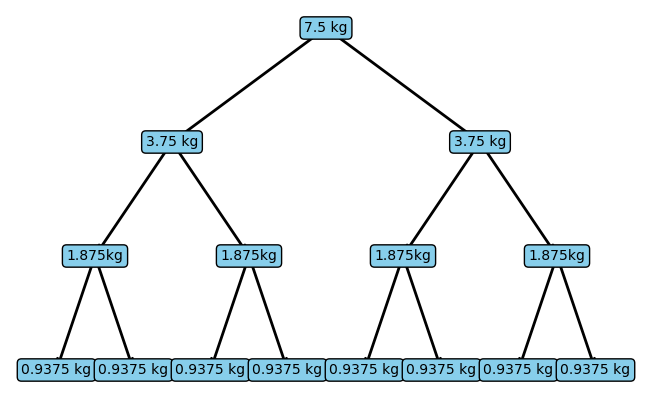
\includegraphics[width=0.9\textwidth]{figures/diagrama_jones}
    \caption{Diagrama de separação de amostras com o Jones.}
    \label{fig:diagrama_jones}
\end{figure}

A amostra foi separada, com o separador \textit{Jones}, em sacos de aproximadamente 1~kg.
A massa de cada saco está apresentada na Tabela~\ref{tab:massa_sacos}.

\begin{table}[!htbp]
    \centering
    \begin{tabular}{@{}lc@{}}
        \toprule
        \textbf{Amostra} & \textbf{Massa (g)} \\ \midrule
        \textcolor{CornflowerBlue}{A$_{01}$} & \textcolor{CornflowerBlue}{1020,66} \\
        A$_{02}$ & 836,56 \\
        A$_{03}$ & 802,66 \\
        \textcolor{YellowOrange}{A$_{04}$} & \textcolor{YellowOrange}{1052,15} \\
        A$_{05}$ & 986,89 \\
        A$_{06}$ & 786,81 \\
        A$_{07}$ & 1138,15 \\
        \textcolor{YellowGreen}{A$_{08}$} & \textcolor{YellowGreen}{1044,50} \\ \midrule
        \textbf{Total} & 7590,38 \\ \bottomrule
    \end{tabular}
    \caption{Massa dos amostras separadas com o \emph{Jones}.}
    \label{tab:massa_sacos}
\end{table}

\marginnote[-0.5cm]{As células destacadas representam as amostras escolhidas para crivagem, que vai ser realizada posteriormente.}

\hrulefill

%%%%%%%%%%%%%%%%%%%%%%%%%%%%%%%%%%%%%%%%%%%%%%%%%%%%%%%%
\pagebreak

\newday{28 Outubro 2024}

Hoje foi realizada a crivagem do material previamente separado.
Escolheu-se, aleatoriamente, três dos oito sacos.
Os sacos escolhidos para crivagem foram os seguintes: A$_{01}$, A$_{04}$ e A$_{08}$; destacados na Tabela~\ref{tab:massa_sacos}.

A série de crivos utilizada para crivagem foi a seguinte:

\begin{minipage}{0.4\textwidth}
    \begin{enumerate}
        \item 0,850~mm
        \item 0,600~mm
    \end{enumerate}
\end{minipage}
\begin{minipage}{0.4\textwidth}
    \begin{enumerate}
        \setcounter{enumi}{2}
        \item 0,425~mm
        \item 0,300~mm
    \end{enumerate}
\end{minipage}

O material foi crivado nos crivos mecânicos\sidenote{Uma particularidade dos crivos mecânicos utilizados é que estes tinham a funcionalidade de definir automaticamente a frequência de vibração de acordo com o peso da coluna de crivos.} durante 30~minutos.
A mesma série de crivos foi utilizada para os três sacos.

Após cada crivagem, a massa das frações de material retido em cada um dos crivos da série de crivagem foi medida e está apresentada na Tabela~\ref{tab:massa_retido_crivagem}:

\begin{table}[!htb]
    \centering
    \begin{tabular}{@{}lccc@{}}
        \toprule
        \multirow{2}{*}{\textbf{Malha (mm)}} & \multicolumn{3}{c}{\textbf{Massa (g)}} \\ \cmidrule(lr){2-4}
         & \multicolumn{1}{c}{\textbf{A$\bm{_{01}}$}} & \multicolumn{1}{c}{\textbf{A$\bm{_{04}}$}} & \textbf{A$\bm{_{08}}$} \\ \hline
        \textbf{0,850} & \multicolumn{1}{c}{4,72} & \multicolumn{1}{c}{4,82} & 4,69 \\
        \textbf{0,600} & \multicolumn{1}{c}{4,26} & \multicolumn{1}{c}{4,48} & 4,43 \\
        \textbf{0,425} & \multicolumn{1}{c}{7,06} & \multicolumn{1}{c}{8,15} & 9,65 \\
        \textbf{0,300} & \multicolumn{1}{c}{30,65} & \multicolumn{1}{c}{31,53} & 41,93 \\
        \textbf{Infra} & \multicolumn{1}{c}{973,37} & \multicolumn{1}{c}{1002,44} & 982,95 \\ \midrule
        \textbf{\bm{$\sum$}}& \multicolumn{1}{c}{\textbf{1020,06}} & \multicolumn{1}{c}{\textbf{1051,42}} & \textbf{1043,65} \\ \bottomrule
    \end{tabular}
    \caption{Massa de material retido em cada crivo após a crivagem.}
    \label{tab:massa_retido_crivagem}
\end{table}

\newpara

Foi efetuada uma análise granulométrica do material retido em cada crivo.
A curva granulométrica está apresentada na Figura~\ref{fig:curva_granulometrica}.
\begin{figure}[!htb]
    \centering
    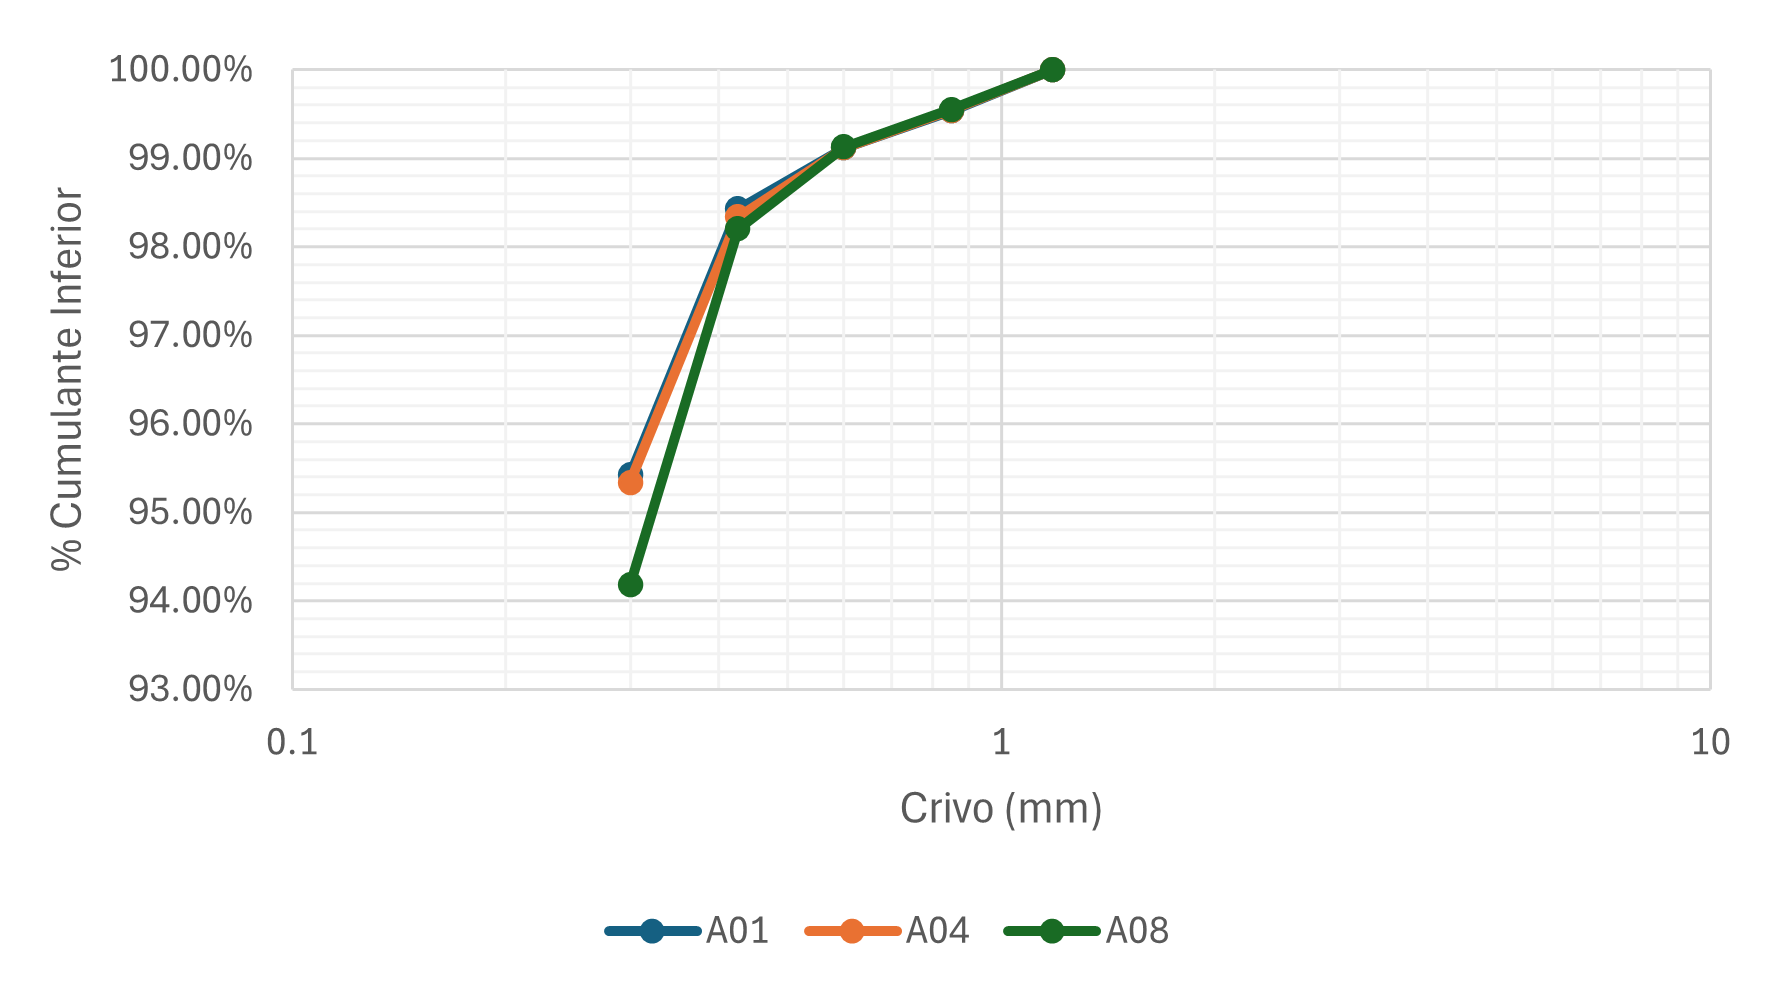
\includegraphics[width=0.9\linewidth]{figures/curva_granulometrica}
    \caption{Curva granulométrica.}
    \label{fig:curva_granulometrica}
\end{figure}

Como existe muito pouco material acima do calibre 0,300~mm (<~5~\%), juntou-se todas as frações de material novamente e vai-se realizar medições no granulómetro laser.

\hrulefill
\pagebreak
%%%%%%%%%%%%%%%%%%%%%%%%%%%%%%%%%%%%%%%%%%%%%%%%%%%%%%%%

\newday{30 Outubro 2024}

\newthought{Granulómetro Laser} \href{https://www.malvernpanalytical.com/en/support/product-support/mastersizer-range/mastersizer-2000}{Malvern Mastersizer 2000}

\marginnote{Um granulómetro laser utiliza a difração da luz laser para medir a distribuição dos tamanhos das partículas numa amostra. Este tipo de análise é particularmente útil porque permite uma análise rápida, precisa e repetível.}

Continuando o trabalho, as frações das amostras previamente crivadas foram colocadas todas na sua forma original (amostra tal-qual de $\approx$~1~kg) para se analisar a granulometria dos 8~sacos de material, com auxílio do granulómetro laser - Figura~\ref{fig:granulometro_laser}.

\begin{figure}[!htb]
    \centering
    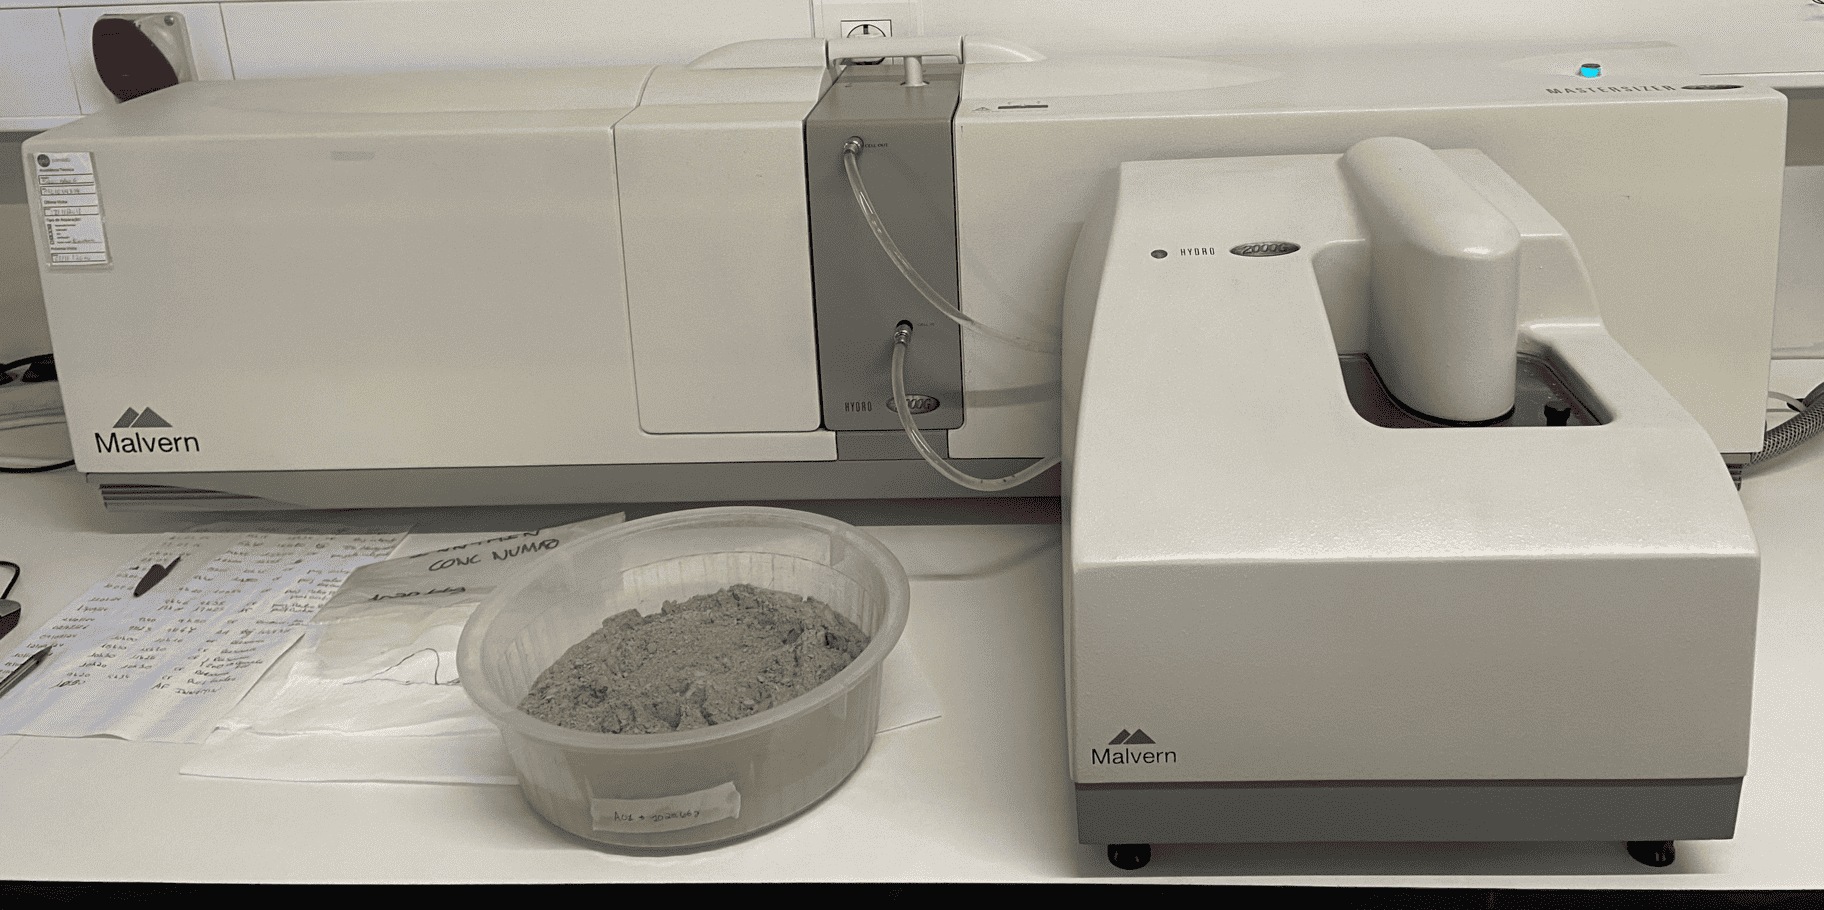
\includegraphics[width=0.75\linewidth]{figures/granulometro_laser}
    \caption{Granulómetro laser Malvern Mastersizer 2000.}
    \label{fig:granulometro_laser}
\end{figure}

Começou-se por analisar a amostra A$_{01}$\sidenote[][-0.25cm]{As amostras foram analisadas separadamente, mas com os resultados obtidos de todas as subamostras poderemos generalizar para a amostra tal-qual ($\approx$~15~kg).}.
A primeira análise foi feita com a amostra seca (ou seja, foi colocada no granulómetro sem estar misturada em água), de forma a avaliar a distribuição do tamanho das partículas.
Verificou-se que havia partículas ainda agregadas\sidenote{Como estamos a trabalhar com material de calibre muito fino, é normal haver agregação de partículas. Isto pode ser combatido com uma agitação forte; uso de ultra-som ou mistura prévia em água para desagregar.}.

Limpou-se o granulómetro e fez-se outra análise desta vez tendo misturado a amostra em água para evitar a agregação das partículas.
Mesmo assim, era possível melhorar ainda mais os resultados e portanto utilizou-se a opção de ultra-som para promover ainda mais a desagregação das partículas.

Visto que com uma mistura prévia em água e com a utilização da opção de ultra-som do granulómetro obtiam-se os melhores resultados, os restantes sacos foram analisados com estas parametrizações.
Sendo que, antes de se ativar o ultra-som\sidenote{A utilização do ultra-som, se for possível, deve ser evitada pois como as partículas são muito finas pode promover a fragmentação e resultar em análises erradas que não refletem a verdadeira composição da amostra.} realizou-se sempre uma análise apenas com a mistura prévia em água.

As análises foram identificadas da seguinte forma:
\begin{itemize}
    \item[-] \texttt{A0n}, sendo \texttt{n} o número da amostra, para análises sem mistura prévia em água e sem ultra-som;
    \item[-] \texttt{A0n-REP}, para análise com mistura prévia em água e sem ultra-som;
    \item[-] \texttt{A0n-REP2}, para análise com mistura prévia em água e com ultra-som.
\end{itemize}

\marginnote[-0.5cm]{Para cada análise foram guardados ficheiros distintos com uma curva granulométrica e com uma curva de distribuição de calibres, \texttt{A0n-REP2-CUM} e \texttt{A0n-REP2-FREQ}, respetivamente.}

Os dados das análises foram guardados para uso posterior.

\hrulefill
\pagebreak

%%%%%%%%%%%%%%%%%%%%%%%%%%%%%%%%%%%%%%%%%%%%%%%%%%%%%%%%

\newday{31 Outubro 2024}\label{day:31-outubro-2024}

\begin{marginfigure}[3\baselineskip]
    \centering
    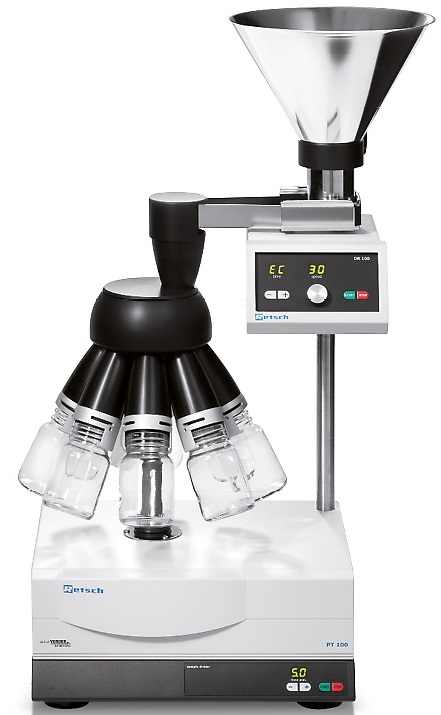
\includegraphics[width=0.55\linewidth]{figures/divisor_de_amostras_retsch}
    \caption{Divisor de amostras \href{https://www.retsch.pt/pt/produtos/assistencia/amostradores/pt-100/}{PT 100}.}
    \label{fig:divisor_de_amostras_retsch}
\end{marginfigure}

Uma fez realizada a análise granulométrica no granulómetro laser, iremos dar continuação à amostragem.
O próximo passo será dividir as amostras de 1~kg em sub-amostras de, aproximadamente 0,250~g - deveremos ter no máximo 250~g e no mínimo 200~g.

Para esta divisão foi utilizado o divisor de amostras apresentado na Figura~\ref{fig:divisor_de_amostras_retsch}.
Este equipamento em específico, divide a amostra em 8~partes iguais.
Portanto, das nossas amostras de $\approx$~1~kg iremos obter 8 sub-amostras de $\approx$~0,125~kg.
Como queremos que as nossas sub-amostras tenham $\approx$~0,250~kg, iremos juntar os frascos resultantes da divisão 2~a~2.

O funcionamento do divisor de amostras é bastante simples e direto.
Coloca-se os frascos, liga-se o equipamento, liga-se o alimentador e coloca-se a amostra (pouco a pouco para prevenir entupimentos) no funil do alimentador\sidenote{O divisor de amostras conta com o alimentador \href{https://www.retsch.pt/pt/produtos/assistencia/alimentadores/}{DR 100} que promove a alimentação contínua de material ao divisor.}.
O divisor faz o resto do trabalho, dividindo a amostra em 8~sub-amostras praticamente iguais.

Das 8~sub-amostras obtidas em cada uma das divisões, constitui-se sacos de $\approx$~0,250~kg, juntando os frascos 2~a~2.
As massas de cada uma das sub-amostras está apresentada na tabela seguinte:

\begin{table*}[ht]
\centering
    \begin{tabular}{@{}lcccccccc@{}}
        \toprule
        \textbf{Sub-amostras (g)} & \textbf{A\bm{$_{01}$}} & \textbf{A\bm{$_{02}$}} & \textbf{A\bm{$_{03}$}} & \textbf{A\bm{$_{04}$}} & \textbf{A\bm{$_{05}$}} & \textbf{A\bm{$_{06}$}} & \textbf{A\bm{$_{07}$}} & \textbf{A\bm{$_{08}$}} \\ \hline
        \textbf{A\bm{$_{0\text{n.}1}$}} & 254,44 & 207,90 & 200,00 & 262,99 & 243,20 & 196,06 & 283,14 & 264,14 \\
        \textbf{A\bm{$_{0\text{n.}2}$}} & 253,67 & 208,76 & 202,18 & 262,30 & 245,76 & 192,84 & 286,50 & 260,05 \\
        \textbf{A\bm{$_{0\text{n.}3}$}} & 254,76 & 210,29 & 200,52 & 262,23 & 250,16 & 198,40 & 284,01 & 257,18 \\
        \textbf{A\bm{$_{0\text{n.}4}$}} & 254,22 & 209,50 & 198,21 & 262,28 & 246,06 & 198,43 & 282,14 & 259,72 \\ \midrule
        \textbf{\bm{$\sum$}} & 1017,09 & 836,45 & 800,91 & 1049,80 & 985,18 & 785,73 & 1135,79 & 1041,09 \\ \bottomrule
    \end{tabular}
\end{table*}

\newpara

Uma vez divididas as sub-amostras, iremos escolher um dos sacos de $\approx$~250~g proveniente da divisão de cada um dos 8 sacos de $\approx$~1~kg.
Estas 8 sub-amostras irão ser analisadas no FRX\sidenote{A fluorescência de raios X (FRX) é uma técnica rápida e não destrutiva amplamente usada para determinar a composição elementar de um material que requer apenas uma preparação mínima da amostra.} para determinar a composição química das amostras.
Como o teor em \ce{Au} deve ser muito pequeno, ele não será determinado por esta análise, obteremos apenas os elementos em maior quantidade.

Foram escolhidas as amostras A$_{01.1}$, A$_{02.3}$, A$_{03.2}$, A$_{04.3}$, A$_{05.3}$, A$_{06.4}$, A$_{07.4}$ e A$_{08.3}$ para serem analisadas no FRX\@.

\begin{marginfigure}[1\baselineskip]
    \centering
    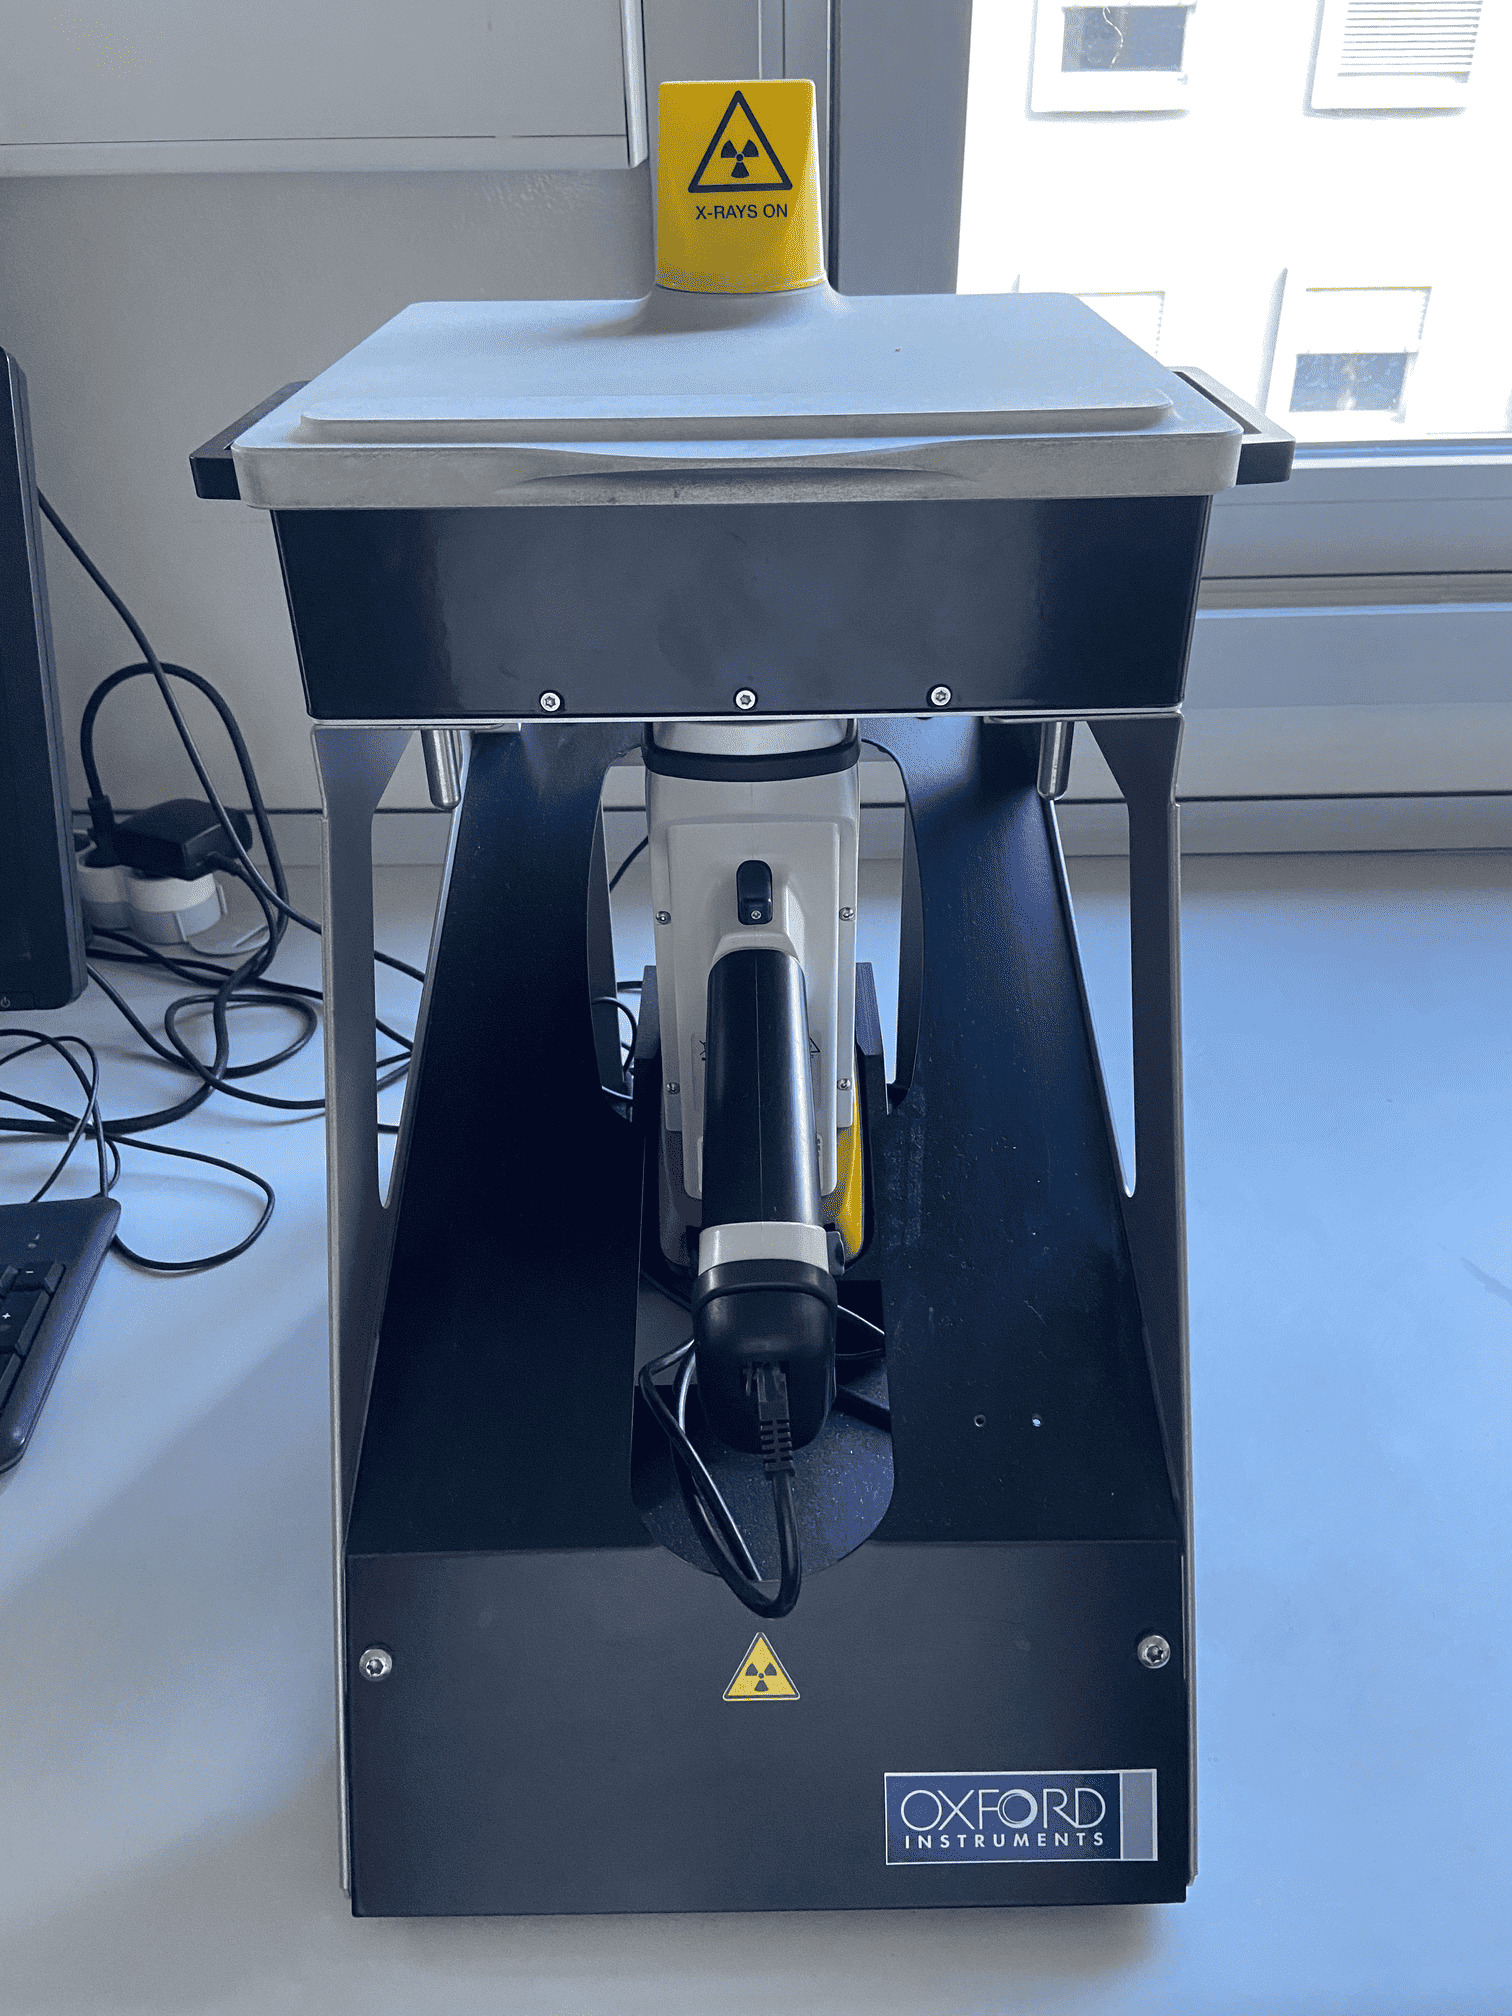
\includegraphics[width=0.7\linewidth]{figures/FRX}
    \caption{Equipamento FRX utilizado.}
    \label{fig:equipamento_frx}
\end{marginfigure}

O funcionamento do equipamento FRX é bastante simples, basta colocar a amostra dentro do equipamento, fechar bem a porta e acionar o gatilho para começar a análise.
Foram realizados cinco ``tiros'' por amostra, com um tempo de análise de 30~segundos em cada tiro.
No fim de cada tiro, foi-se alterando a posição da amostra dentro do equipamento, para que fossem analisadas diferentes partes da amostra de forma a que os resultados sejam representativos.

Os resultados das análises foram descarregados em formato \texttt{.csv}.
Foi necessário trabalhar o ficheiro descarregado para ser possível analisar os dados.
Dessa forma, escreveu-se o seguinte código em Python:

\marginnote{A linha 1 importa o \emph{pandas}, uma biblioteca necessária. A linha 3 permite ler o ficheiro \texttt{.csv} como um \emph{pandas dataframe}. A linha 5 define as colunas que irão ser removidas - são referentes a informações fornecidas pelo equipamento FRX que não nos interessam. A linha 8 remove as colunas especificadas anteriormente. A linha 10 remove as colunas que contém o desvio padrão (se for necessário será calculado posteriormente) e as colunas que não contém informação (elementos químicos não presentes). A linha 12 guarda o ficheiro com as alterações, convertendo-o para Excel.}

\lstinputlisting[language=Python,label={lst:python_code}]{code/tratamento_dados_frx.py}

Os dados irão ser posteriormente analisados.

\hrulefill

%%%%%%%%%%%%%%%%%%%%%%%%%%%%%%%%%%%%%%%%%%%%%%%%%%%%%%%%

\newday{6 Novembro 2024}

Hoje foram refeitas as análises FRX para as amostras \texttt{A01.1}, \texttt{A03.2}, \texttt{A05.3} e \texttt{A08.3}.
Os valores destas análises serão adicionados (substituídos) aos dados obtidos no dia~\nameref{day:31-outubro-2024}.

A necessidade de refazer as análises para estas amostras assenta no facto de o equipamento não ter feito leituras de alguns elementos em alguns dos 5~tiros realizados.
Portanto, é necessário refazer a análise FRX para estas amostras para que a média, que vai ser calculada, seja correta e que os resultados sejam representativos.

\hrulefill
%%%%%%%%%%%%%%%%%%%%%%%%%%%%%%%%%%%%%%%%%%%%%%%%%%%%%%%%

\newday{7 Novembro 2024}

Hoje foi feita a preparação para fazer a digestão ácida.
Para isso foi escolhida, aleatoriamente, uma sub-amostra de $\approx$~250~g para este procedimento.
Foi escolhida a amostra \texttt{A08.3}, com 257,18~g.

Como vão ser necessários apenas 50~g de amostra, a \texttt{A08.3} foi colocada no divisor de amostras - o mesmo da Figura~\ref{fig:divisor_de_amostras_retsch}.

Do divisor de amostras obteu-se 54,15~g que foi depois dividido em cinco copos, cada um com aproximadamente 10~g.
Estes cinco copos foram depois colocados na mufla.
A mufla foi programada para aquecer até 700~\graus, manter os 700~\graus \, durante 1~hora e depois desligar-se automaticamente.
As amostras ficam a arrefecer dentro da mufla até ao dia seguinte.
\begin{marginfigure}
    \centering
    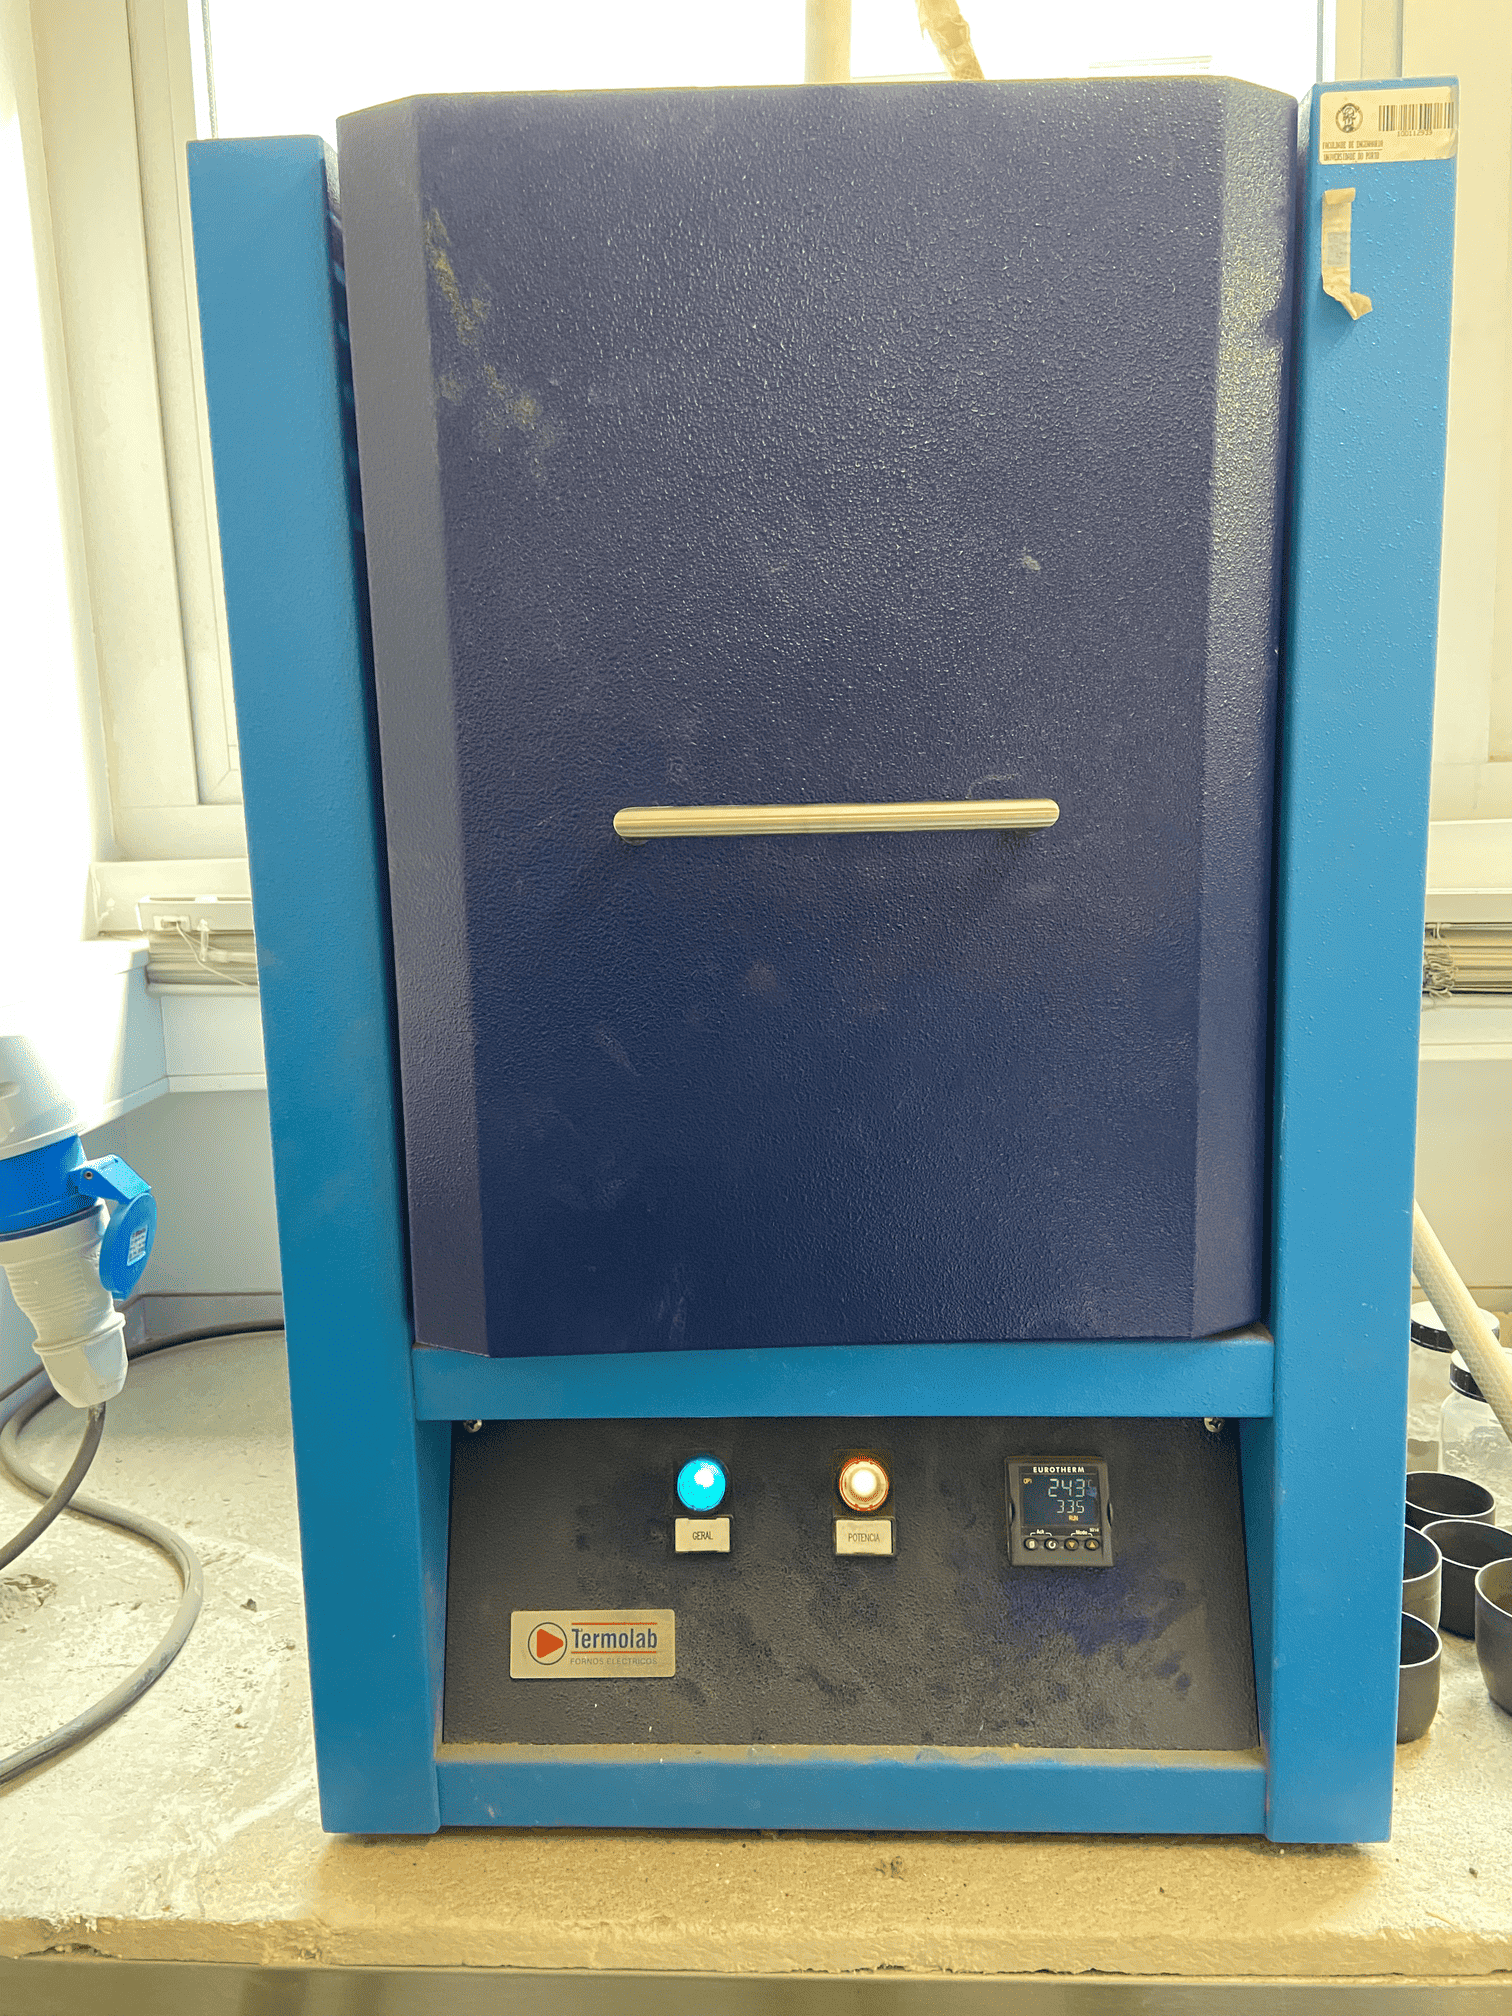
\includegraphics[width=0.7\textwidth]{figures/Mufla}
    \caption{Mufla utilizada para aquecer a amostra.}
    \label{fig:mufla}
\end{marginfigure}

No dia seguinte, com a amostra já arrefecida, será realizada a digestão ácida, sendo que o procedimento será posteriormente explicado.

\hrulefill
%%%%%%%%%%%%%%%%%%%%%%%%%%%%%%%%%%%%%%%%%%%%%%%%%%%%%%%%
%\newday{5 Novembro 2024}
%
%\subsection{Estratégia de Tratamento dos Dados de FRX}\label{subsec:estrategia-tratamento-dados-frx}
%
%O FRX forneceu-nos um ficheiro \texttt{.csv} que continha os resultados das análises efetuadas.
%Esse ficheiro continha valores de concentração de diversos elementos químicos para cada um dos 5 tiros em cada uma das sub-amostras.
%
%O tratamento dos dados é necessário e vão consistir nas seguintes etapas:
%\begin{enumerate}
%    \item Análise exploratória inicial:
%    \begin{enumerate}
%        \item Verificar valores médios e variabilidade: analisar a média e o desvio padrão nos cinco tiros de cada amostra;
%        \item Visualização dos dados: construção de gráficos de bigodes (\emph{box plots}) para cada elemento em cada amostra.
%        \begin{marginfigure}
%            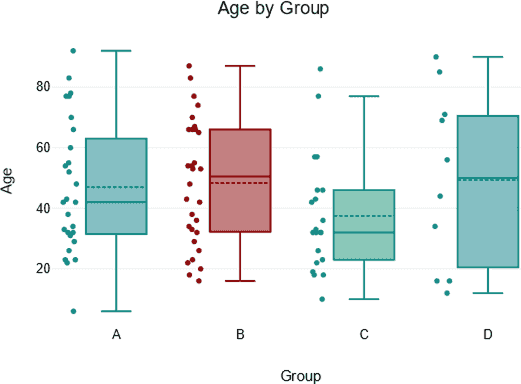
\includegraphics[width=\linewidth]{figures/exemplo_boxplot}
%            \caption{Exemplo de um gráfico de bigodes.}
%            \label{fig:boxplot_example}
%        \end{marginfigure}
%    \end{enumerate}
%    \item Cálculo de Estatísticas Descritivas:
%    \begin{enumerate}
%        \item Para cada elemento de cada amostra, calcular o valor da média geral e do desvio padrão entre os tiros.
%        A média geral representa o valor médio do elemento para a amostra, enquanto o desvio padrão mostra a variabilidade entre os tiros;
%        \item Calcular o coeficiente de variação (CV):
%        \marginnote[0.5cm]{
%            \begin{equation*}
%            CV = \frac{\text{desvio padrão}}{\text{média}}\times 100
%            \end{equation*}
%        }
%        O CV indica a variabilidade em relação à média e é útil para comparar a consistência de diferentes elementos.
%    \end{enumerate}
%    \item Análise de Outliers:
%    \begin{enumerate}
%        \item Analisar os outliers para cada elemento em cada amostra.
%        Dependendo da dispersão observada, identificar tiros atípicos (por exemplo, valores que se afastam mais de 2 ou 3 desvios padrão da média);
%        \item Decidir se esses outliers devem ser mantidos ou removidos, considerando fatores como a homogeneidade da amostra e a precisão do FRX\@.
%    \end{enumerate}
%    \item Cálculo da média Representativa e Intervalos de Confiança:
%    \begin{enumerate}
%        \item Calcular a média representativa final para cada elemento em cada amostra considerando os cinco tiros (ou menos, se tiver removido os outliers);
%        \item Construir intervalos de confiança para a média de cada elemento em cada amostra.
%        Para amostras pequenas (como 5 tiros), o intervalo de confiança é uma boa medida da variabilidade dos dados.
%    \end{enumerate}
%    \end{enumerate}
%
%Exemplo de como organizar os dados:
%\begin{table}[!htb]
%    \centering
%    \caption{Organização dos dados.}
%    \label{tab:organizacao-dos-dados}
%    \begin{tabular}{@{}lccccc@{}}
%        \toprule
%        \textbf{Amostra} & \textbf{Elemento} & \bm{$\overline{x}$} & \bm{$\sigma$} & \textbf{CV} & \textbf{Int. Conf.}  \\ \midrule
%        A01 & \ce{Fe} & xx.x & x.x & x.x & [xx.x; xx.x] \\
%        A02 & \ce{Cu} & xx.x & x.x & x.x & [xx.x; xx.x] \\
%        \ldots & \ldots & \ldots & \ldots & \ldots & \ldots \\
%        \bottomrule
%    \end{tabular}
%\end{table}
%
%\marginnote{Na Tabela~\ref{tab:organizacao-dos-dados}, $\overline{x}$ representa a média e $\sigma$ o desvio padrão.}
%
%\subsection{Tratamento dos Dados de FRX}\label{subsec:tratamento-dos-dados-de-frx}

%%%%%%%%%%%%%%%%%%%%%%%%%%%%%%%%%%%%%%%%%%%%%%%%%%%%%%%%